\documentclass{beamer}
\usepackage{tikz,comment,fontawesome,hyperref}
\usetikzlibrary{calc}
\title{Towards ICN-based signaling network for 6G}
\author{TungTQ}

\begin{document}
\begin{frame}
  \frametitle{NFs direct communication SBA}
  \begin{itemize}
    \item {Direct communication between NFs (release 15): small scale deployments
    \begin{itemize}
      \item control plane is shared by multiple types of traffic with diverse priorities
      \item potential bottleneck for requests to NRF
    \end{itemize}
    }

  \end{itemize}
  \center
  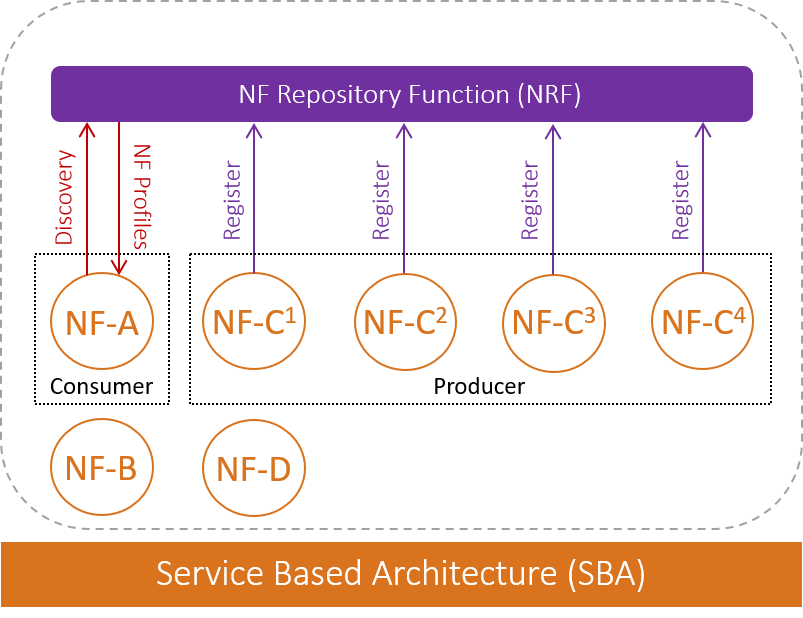
\includegraphics[width=0.7\textwidth]{images/sba-nrf}
\end{frame}
\begin{frame}
  \frametitle{Service Communication Proxy (SCP)}
  \begin{itemize}
    \item {SCP-based deploymen becomes a norm $\rightarrow $ SCP is introduced to release 16
    \begin{itemize}
    
    
    \item Delegated discovery and selection
    \item Load balancing \& alternate routing
    \item SBI traffic feed for monitoring
    \item Rate limiting; Congestion control
    \end{itemize}
    }
    \center
  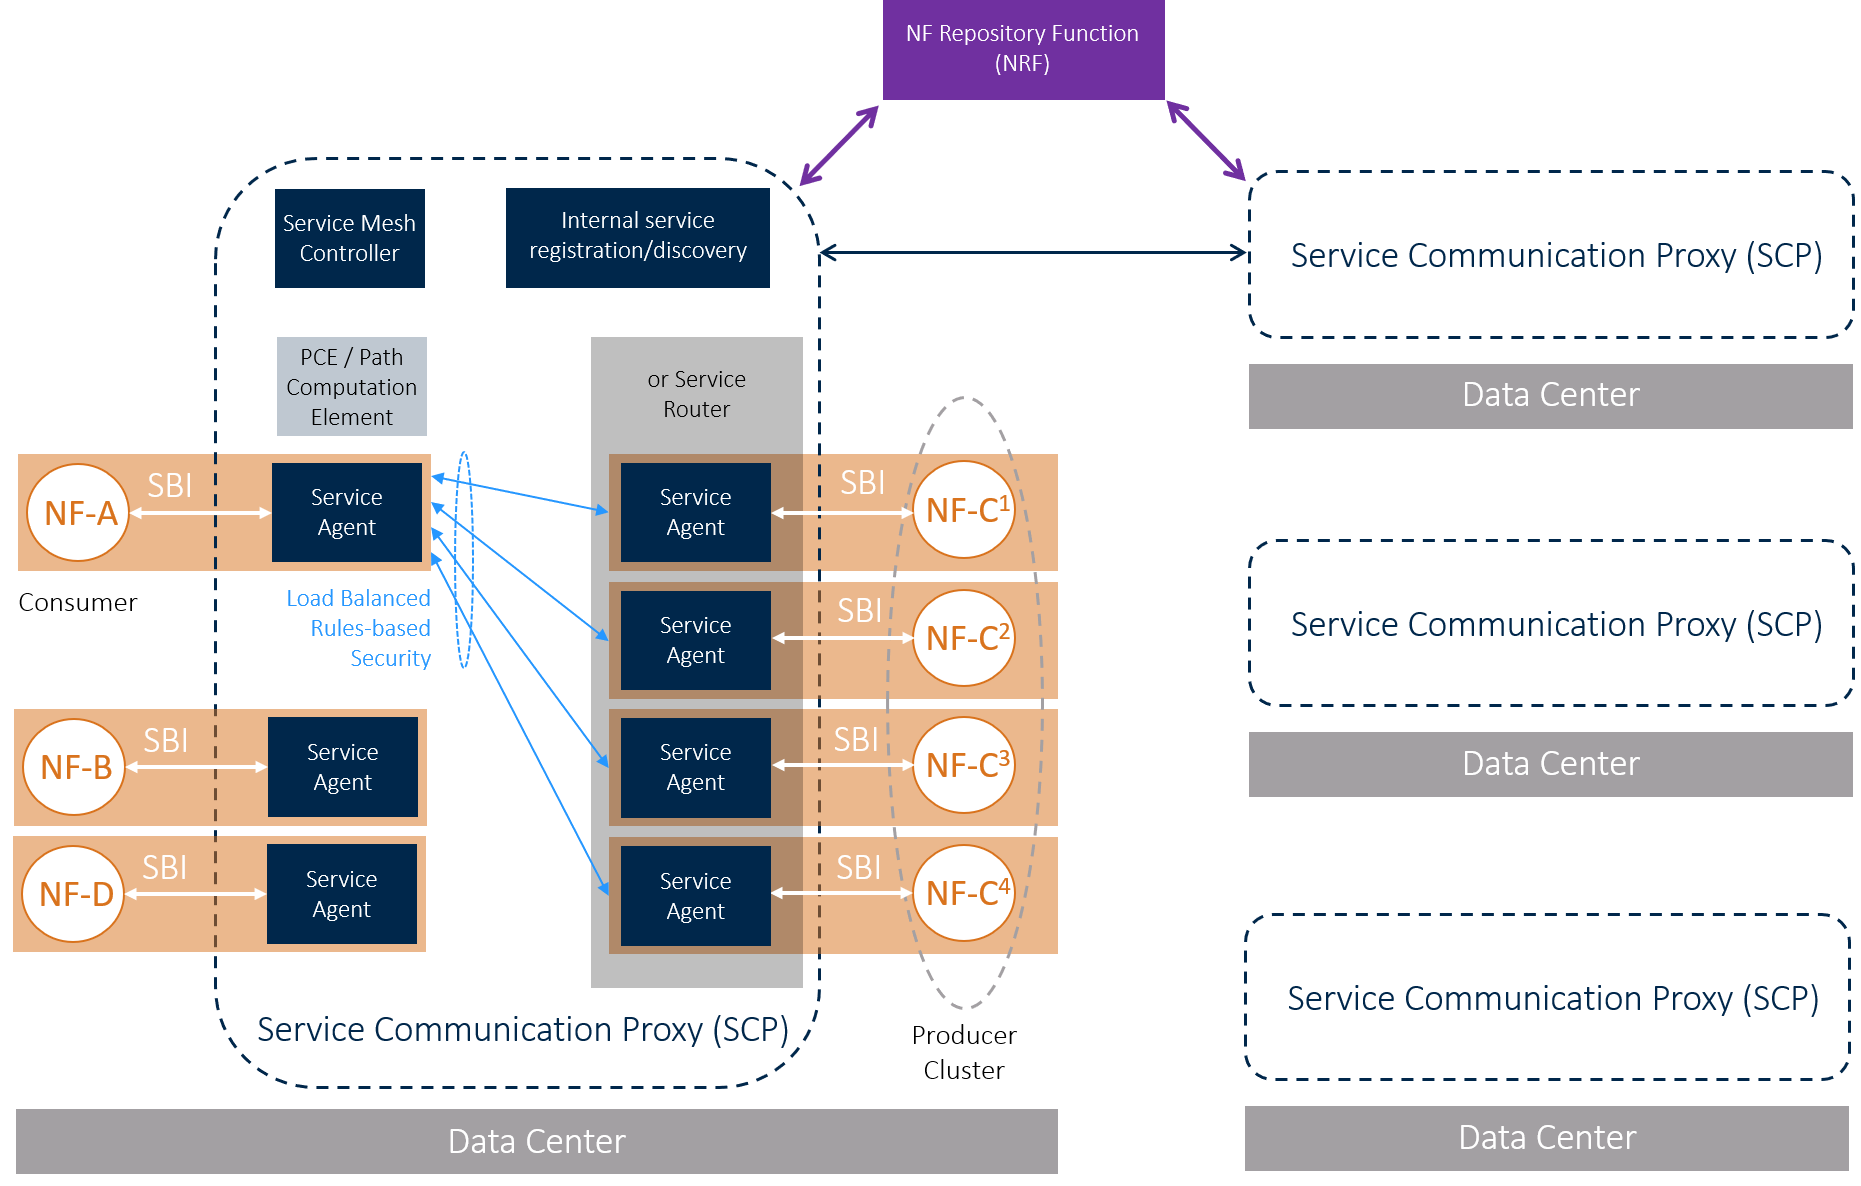
\includegraphics[width=0.7\textwidth]{images/sba-scp}
  \end{itemize}
  
\end{frame}
\begin{frame}
\frametitle{Benefit}
\begin{itemize}
  \item Ease of operation; Massive scalability of signaling transactions
  \item Enhance Reliency: alterate routing, circuit breaking, rate limiting
  \item Multiple domain network (carrier-carrier, vertical industries)
  \item Canary upgrade for NFs
  \item Security
\end{itemize}
\end{frame}

\begin{frame}
  \frametitle {SBA adoption}
  \begin{itemize}
    \item {Loosely couple services, flexibility in service oriented control plan \textcolor{green}{\faCheckCircle}}
    \item {Modularity, in operational and management independence \textcolor{green}{\faCheckCircle}}
    \item {True cloud native \textcolor{red}{\faClose}}
    \item {Extensibility, services interact with lightweight service based APIs \textcolor{red}{\faClose}}
    \item {Openess to 3rd party via north APIs \textcolor{red}{\faClose}}
  \end{itemize}
\end{frame}

\begin{frame}
  \frametitle{Evolution towards a True End-to-End Service Based Architecture}
  \begin{itemize}
    \item{How can the
6G business be transformed from closed connectivity-driven business to novel open sustainable ecosystemic business models in 6G}
    \item Need an integration fabric (SCP was a single domain integration fabric)
  \end{itemize}
  \center
  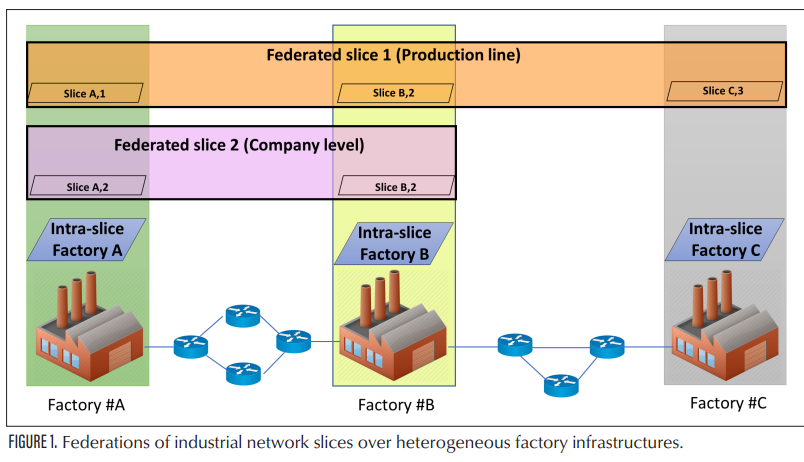
\includegraphics[width=0.8\textwidth]{images/fabric}
\end{frame}

\begin{comment}
\begin{frame}
  \frametitle{Why ICN-based signaling network?}
  \begin{center}
  
  
  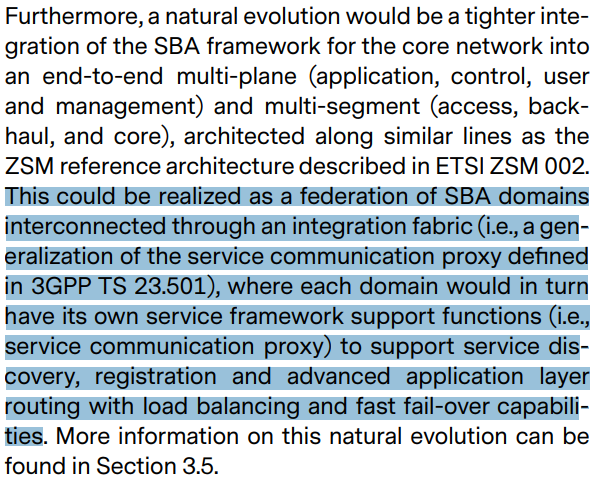
\includegraphics[width=0.45\textwidth]{images/scp-net}%
  
  \footnotesize{\textit{Whitepaper on 6G Networking (6G Falgship University)}}
  \end{center}
  
  \small{
  \begin{itemize}
    \item Named-based routing SCP was one of the option in Release 16
   
    \item {Http/tcp based SBA is one of realizations, there can be other options (gRPC, ICN, pub/sub system) which may have better performance}
    \item {Pub/sub system can be a important component $\rightarrow$ ICN natively suitable}
    \item Ease of operation (name-based management)
    \item Name-based security management instead of connection-based security management

  \end{itemize}
  }
\end{frame}

\end{comment}

\begin{frame}
  \frametitle{Requirements for the integration fabric}
  \begin{itemize}
    \item {True cloud-native: isolate service identification from its location
    \begin{itemize}
      \item applications/NFs may request service from another NF without knowing its location
      \item $\rightarrow$ simplify application business logic, easy to compose new services
    \end{itemize}
    }
  \end{itemize}
  \begin{center}
  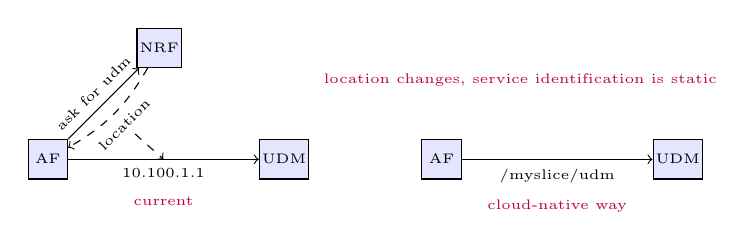
\begin{tikzpicture}[nf/.style={rectangle, draw,inner sep=1pt,fill=blue!10,minimum width=0.5cm, minimum height=0.5cm}]
    \node [nf] at (0,0) (nf1) {\tiny AF};
    \node [nf] at ($(nf1)+(3cm,0)$) (nf2) {\tiny UDM};
    \node [nf] at ($(nf1)+(45:2cm)$) (nf3) {\tiny NRF};
    
    \draw[->] (nf1) -- node[below] (ip) {\tiny 10.100.1.1} (nf2);
    \draw[->] (nf1) -- node[above,sloped]  {\tiny ask for udm} (nf3);
    \draw[->,dashed] (nf3) to[out=-120,in=30] node[pos=0.5,sloped,below] (a) {\tiny location} (nf1);
    \draw[->,dashed] (a) --node[right] {} (ip.north);
    
    \node [nf] at ([xshift=2cm]nf2) (nf4) {\tiny AF};
    \node [nf] at ($(nf4)+(3cm,0)$) (nf5) {\tiny UDM};
    \draw[->] (nf4) -- node[below] (icn) {\tiny /myslice/udm} (nf5);
    \node at ([xshift=1cm,yshift=1cm]nf4) {\tiny \textcolor{purple}{location changes, service identification is static}};
    \node[below] at ([yshift=-5pt]ip) {\tiny \textcolor{purple}{current}};
    \node[below] at ([yshift=-5pt]icn) {\tiny \textcolor{purple}{cloud-native way}};
    
  \end{tikzpicture}
  \end{center}
  
\end{frame}

\begin{frame}
  \frametitle{Requirements for the integration fabric}
  \begin{itemize}
    \item {Support subscribe/notification communication model better
    \begin{itemize}
       \item  having a separated pub/sub system, removing the subscriber management from NFs
       \item multicasting: 1 publisher - many subscribers
    \end{itemize}
    }
  \begin{center}
  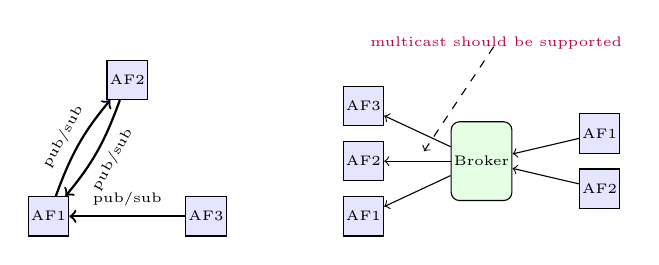
\begin{tikzpicture}[nf/.style={rectangle, draw,inner sep=1pt,fill=blue!10,minimum width=0.5cm, minimum height=0.5cm}]
    \node [nf] at (0,0) (nf1) {\tiny AF1};
    \node [nf] at ($(nf1)+(2cm,0)$) (nf3) {\tiny AF3};
    \node [nf] at ($(nf1)+(60:2cm)$) (nf2) {\tiny AF2};
    \draw [->, thick] (nf1) to[in=-130,out=70] node[above,sloped] {\tiny pub/sub} (nf2); 
    \draw [->, thick] (nf2) to[out=-110,in=50] node[below,sloped] {\tiny pub/sub} (nf1); 
    \draw [->, thick] (nf3) -- node[above,sloped] {\tiny pub/sub} (nf1); 
    
    \node [nf] at ($(nf3)+(2cm,0)$) (nf4) {\tiny AF1};
    \node [nf] at ($(nf4)+(0,0.7cm)$) (nf5) {\tiny AF2};
    \node [nf] at ($(nf5)+(0,0.7cm)$) (nf6) {\tiny AF3};
    \node [rectangle,rounded corners=3pt,inner sep=1pt,draw, fill=green!10,minimum height=1cm] at ($(nf5)+(1.5cm,0)$) (bk) {\tiny Broker};
    \node [nf] at ($(bk)+(1.5cm,0.35cm)$) (nf7) {\tiny AF1};
    \node [nf] at ($(bk)+(1.5cm,-0.35cm)$) (nf8) {\tiny AF2};
    \draw[->] (bk) -- (nf6);
    \draw[->] (bk) -- (nf4);
    \draw[->] (bk) -- node (aa) {} (nf5);
    \draw[->] (nf7) -- (bk);
    \draw[->] (nf8) -- (bk);
    \draw[<-, dashed] (aa) -- ++(1cm,1.5cm) node {\tiny \textcolor{purple}{multicast should be supported}};
    
  \end{tikzpicture}
  \end{center}    
    \item {Performance
    \begin{itemize}
       \item {http is an adhoc selection}
    \end{itemize}
    }
  \end{itemize}
\end{frame}
\begin{frame}
  \frametitle{ICN as a candidate}
  \begin{itemize}
    \item {ICN can tick all the boxes}
    \item {Not vanila ICN, but 5g/6g aware version of ICN \begin{itemize}
      \item network status aware (load balancing, fault tolerent, congestion control)
      \item known parties (not public network) $\rightarrow$ support push multicast (pull multicast is native in ICN)
    \end{itemize}
    }
  \end{itemize}
\end{frame}

\begin{frame}
  \frametitle{An example}
  \begin{center}
  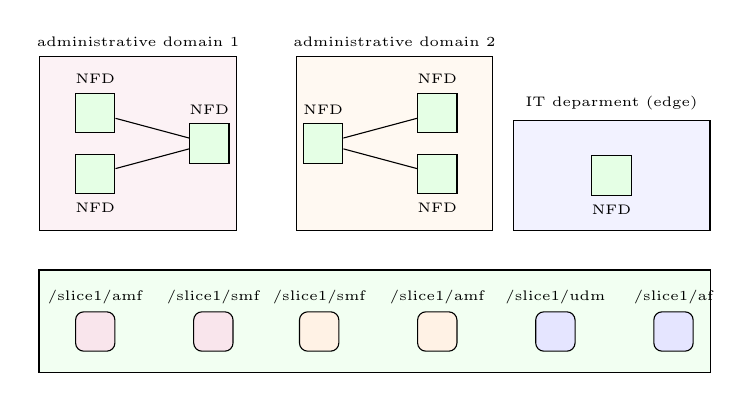
\begin{tikzpicture}[nfd/.style={rectangle,draw=black, inner sep=2pt,minimum width=0.5cm,minimum height=0.5cm, fill=green!10},
  nf/.style={rectangle,rounded corners=3pt,draw=black, inner sep=2pt,minimum width=0.5cm,minimum height=0.5cm, fill=blue!10}]
    \node[rectangle,draw, fill=purple!5, minimum width=2.5cm, minimum height=2.2cm] at (0,0) (dom1) {};
    \node[rectangle,draw, fill=orange!5, minimum width=2.5cm, minimum height=2.2cm] at ([xshift=2cm]dom1.east)(dom2) {};
    \node[rectangle,draw, fill=blue!5,minimum width=2.5cm, minimum height=1.4cm] at ([xshift=1.5cm, yshift=0.7cm]dom2.south east) (dom3){};
    
    \node[nfd] at ([xshift=-10pt]dom1.east) (r1) {};
    \node[nfd] at ($(r1)+(-15:-1.5cm)$) (r2) {};
    \node[nfd] at ($(r1)+(15:-1.5cm)$) (r3) {};
    \draw[-] (r1) -- (r2);
    \draw[-] (r1) -- (r3);
    \node[yshift=5pt] at (r1.north) {\tiny NFD};
    \node[yshift=5pt] at (r2.north) {\tiny NFD};
    \node[yshift=-5pt] at (r3.south) {\tiny NFD};
    
    \node[nfd] at ([xshift=10pt]dom2.west) (r4) {};
    \node[nfd] at ($(r4)+(15:1.5cm)$) (r5) {};
    \node[nfd] at ($(r4)+(-15:1.5cm)$) (r6) {};
    \draw[-] (r4) -- (r5);
    \draw[-] (r4) -- (r6);
    \node[yshift=5pt] at (r4.north) {\tiny NFD};
    \node[yshift=5pt] at (r5.north) {\tiny NFD};
    \node[yshift=-5pt] at (r6.south) {\tiny NFD};

    \node[nfd] at (dom3) (it) {};
    \node[yshift=-5pt] at (it.south) {\tiny NFD};
    
    \node[above] at (dom1.north) {\tiny administrative domain 1};
    \node[above] at (dom2.north) {\tiny administrative domain 2};
    \node[above] at (dom3.north) {\tiny IT deparment (edge)};
    
    \draw[fill=green!5] ([yshift=-0.5cm]dom1.south west) rectangle ([yshift=-1.8cm]dom3.south east);

    \node[nf,fill=purple!10] at ([yshift=-2cm]r3) (nf1) {};
    \node[nf,fill=purple!10] at ($(nf1)+(1.5cm,0)$) (nf2) {};
    \node[nf,fill=orange!10] at ([yshift=-2cm]r6) (nf3) {};
    \node[nf,fill=orange!10] at ($(nf3)+(-1.5cm,0)$) (nf4) {};
    
    \node[nf] at ($(nf3)+(1.5cm,0)$) (nf5) {};
    \node[nf] at ($(nf5)+(1.5cm,0)$) (nf6) {};
    
    
    \node at ([yshift=5pt]nf1.north) {\tiny /slice1/amf};
    \node at ([yshift=5pt]nf2.north) {\tiny /slice1/smf};
    \node at ([yshift=5pt]nf3.north) {\tiny /slice1/amf};
    \node at ([yshift=5pt]nf4.north) {\tiny /slice1/smf};
    \node at ([yshift=5pt]nf5.north) {\tiny /slice1/udm};
    \node at ([yshift=5pt]nf6.north) {\tiny /slice1/af};
    
  \end{tikzpicture}
  \end{center}
\end{frame}

\begin{frame}
  \Large{2022/06/16 meeting $\rightarrow$}
\end{frame}

\begin{frame}
  \frametitle{Microservice architechture}
  \center
  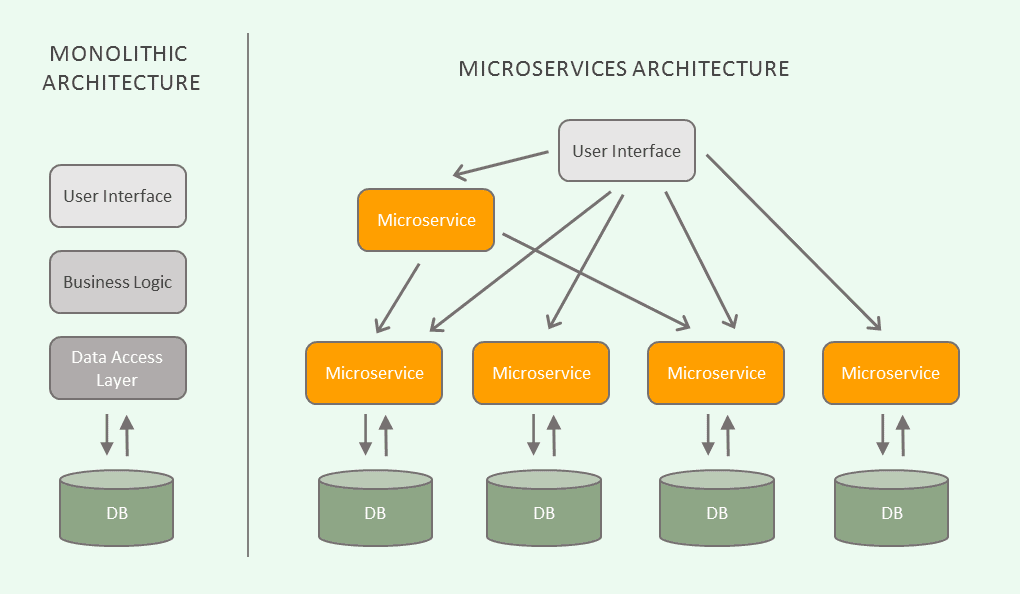
\includegraphics[width=0.9\textwidth]{images/microservice-arch}
  \tiny{\url{https://www.datarobot.com/blog/introduction-to-microservices/}}
\end{frame}


\begin{frame}
  \frametitle{Microservice architechture evolution}
  \center
  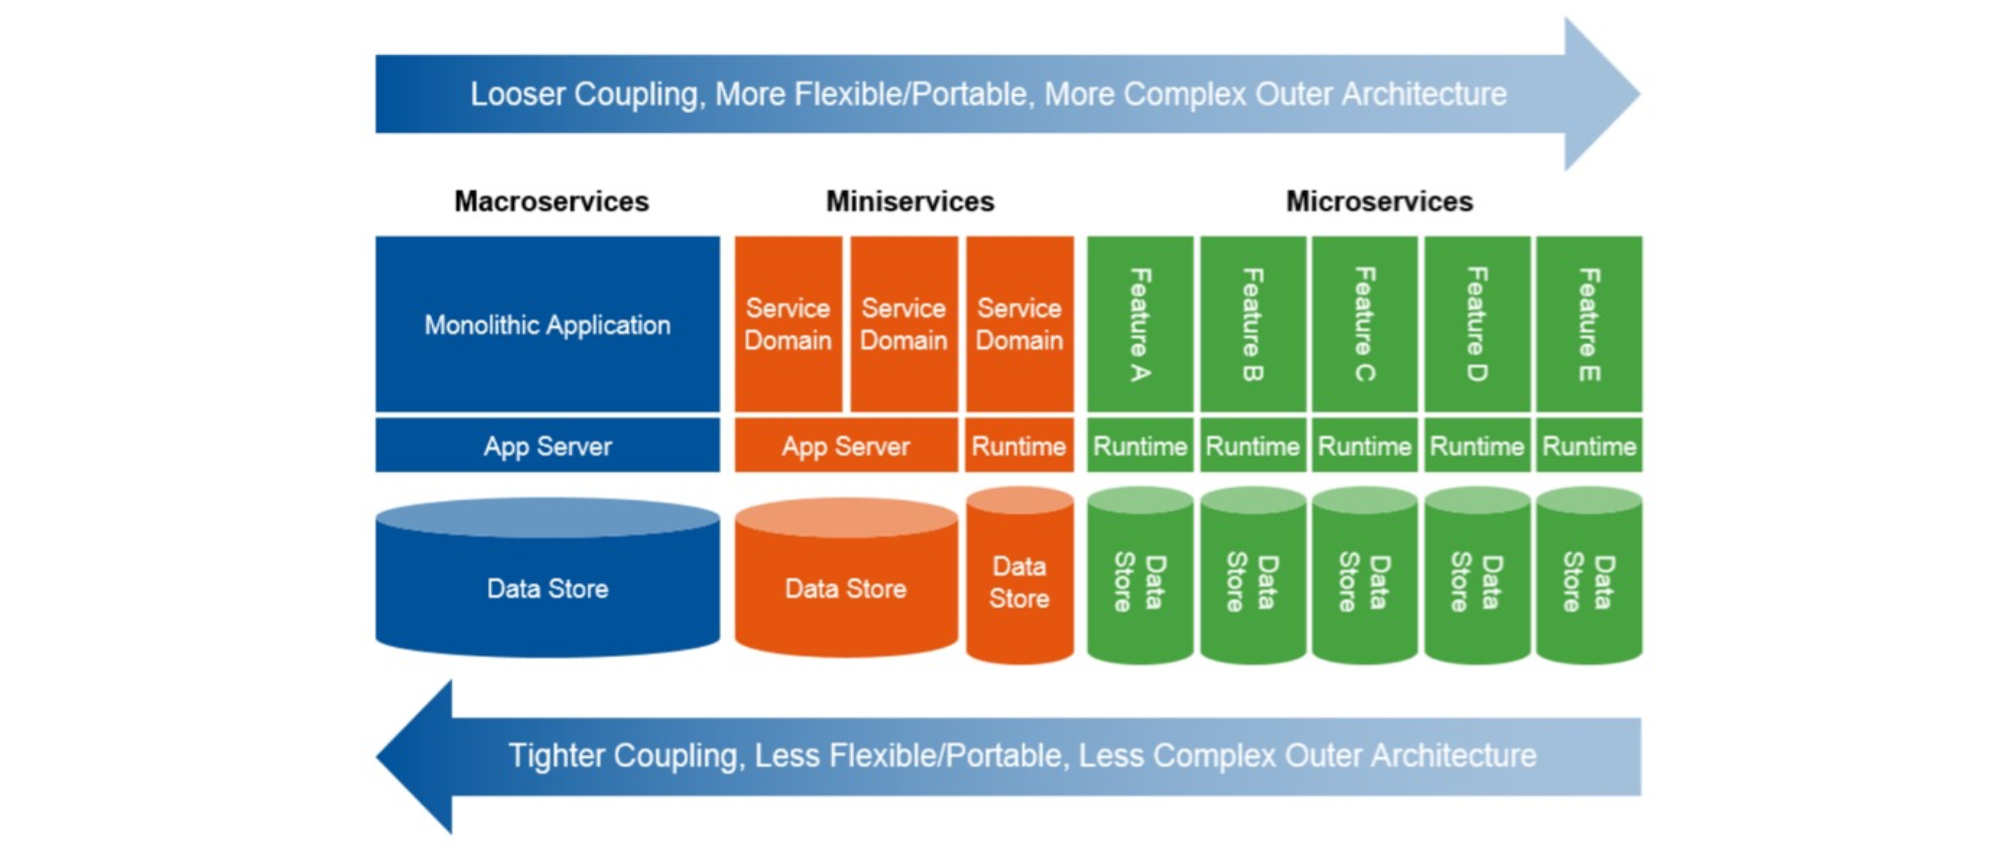
\includegraphics[width=0.9\textwidth]{images/microservice-evolution}
  \tiny{\url{https://www.smartwavesa.com/blog-articles/microservice-architecture-benefits-and-challenges/}}
\end{frame}

\begin{frame}
  \frametitle{Service mesh}
    A service may have multiple instances. Application may consist of hudrends of interconnected services. $\rightarrow$  How to find an instance to request service? $\rightarrow$ Need a service mesh.
    \center
  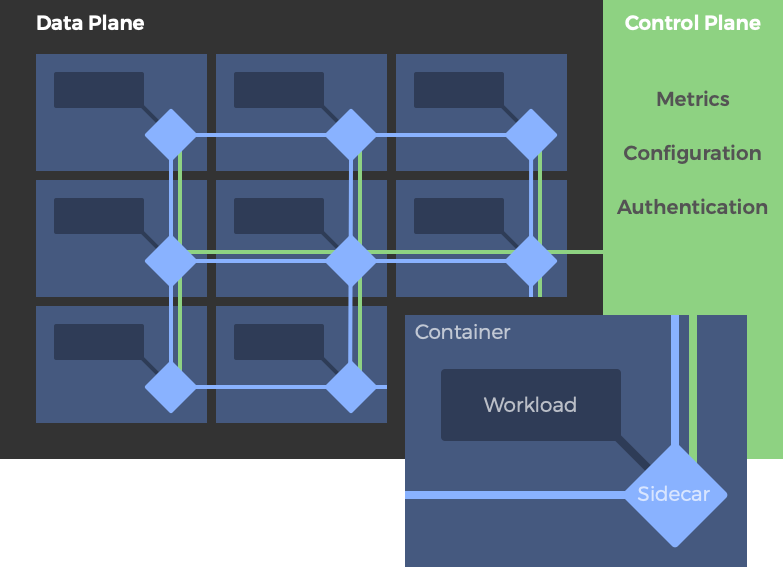
\includegraphics[width=0.8\textwidth]{images/service-mesh}
\end{frame}

\begin{frame}
  \frametitle{Control plane/Data plane (istio service mesh)}
  \center
  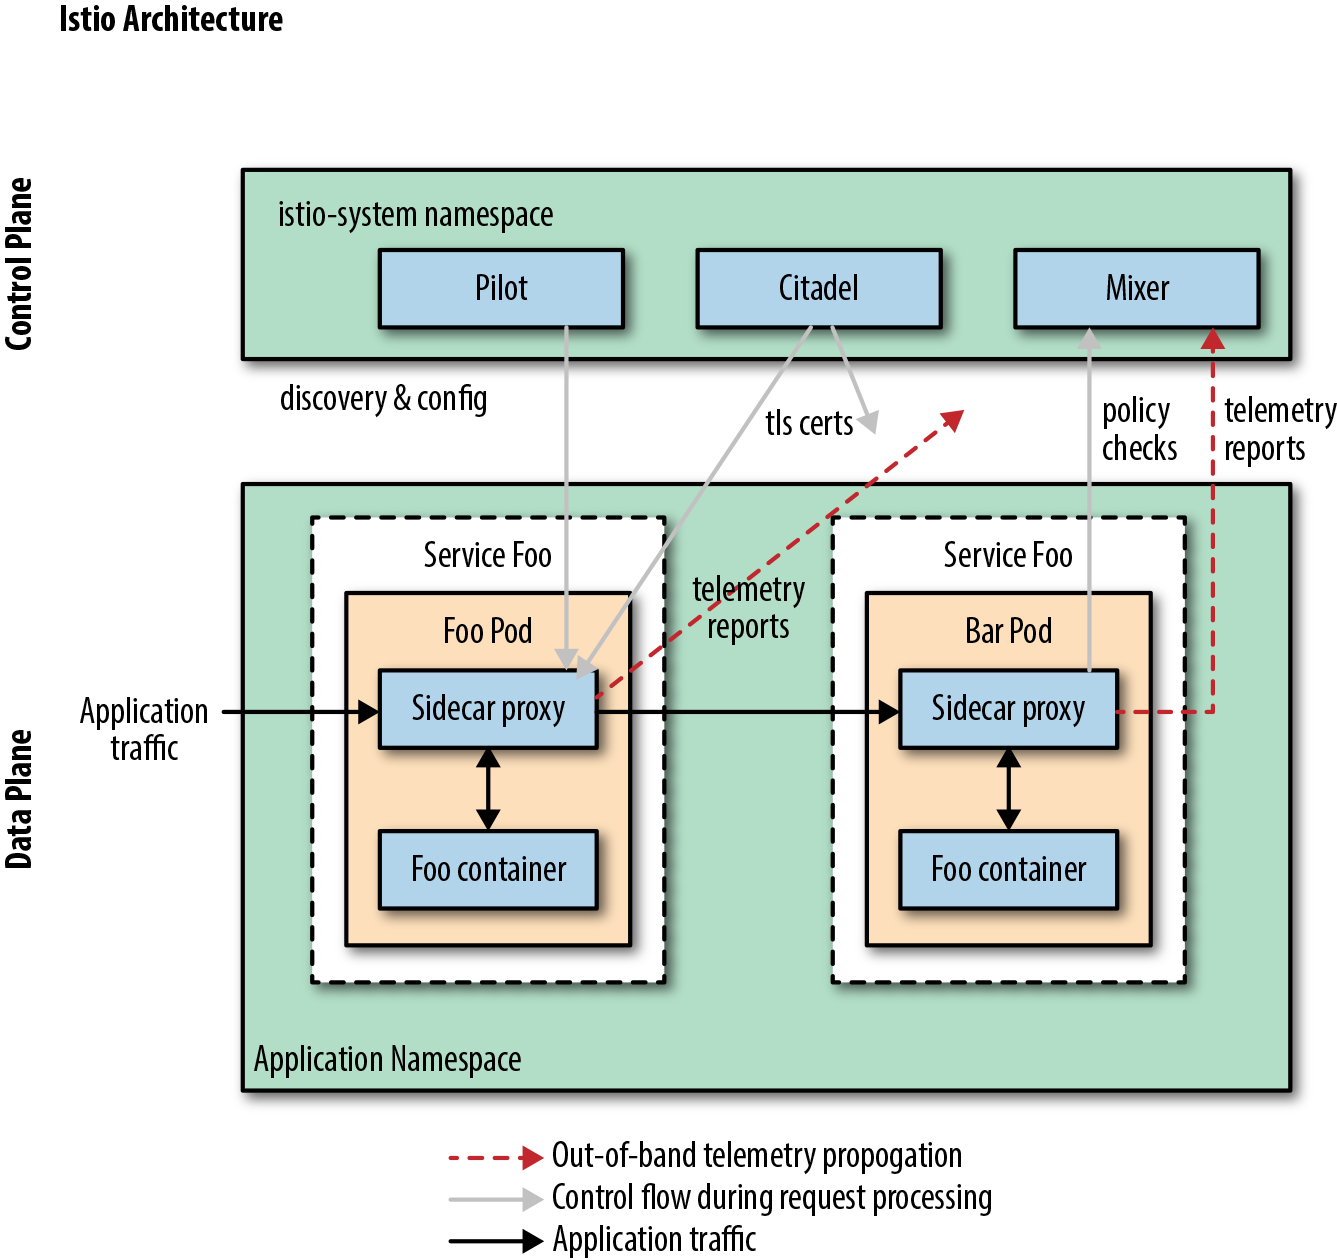
\includegraphics[width=0.8\textwidth]{images/istio-arch}
\end{frame}


\begin{frame}
  \frametitle{Service mesh features}
  \begin{itemize}
    \item  Service discovery: registry and discovery of services    
    \item  Routing: intelligent load balancing and network routing, better health checks, automatic deployment patterns such as blue-green or canary deployments
    \item Resilience: retries, timeouts and circuit breakers
    \item Security: TLS-based encryption including key management
    \item Telemetry: collection of metrics and tracing identifiers
  \end{itemize}
\end{frame}
\begin{frame}
  \frametitle{Benefit/limitations}
  
  Benefits:
  \begin{itemize}
    \item Observability
    \item Traffic Control    
    \item Security
  \end{itemize}
  
  Limitations
  \begin{itemize}
    \item Added complexity
    \item Need expertise
    \item Slowness
    \item Adoption of a platform
  \end{itemize}
  \tiny {source: \url{https://glasnostic.com/blog/service-mesh-istio-limits-and-benefits-part-1}}
\end{frame}

\begin{frame}
  \frametitle{Distributed deployment of NFs in SBA}
  \center
  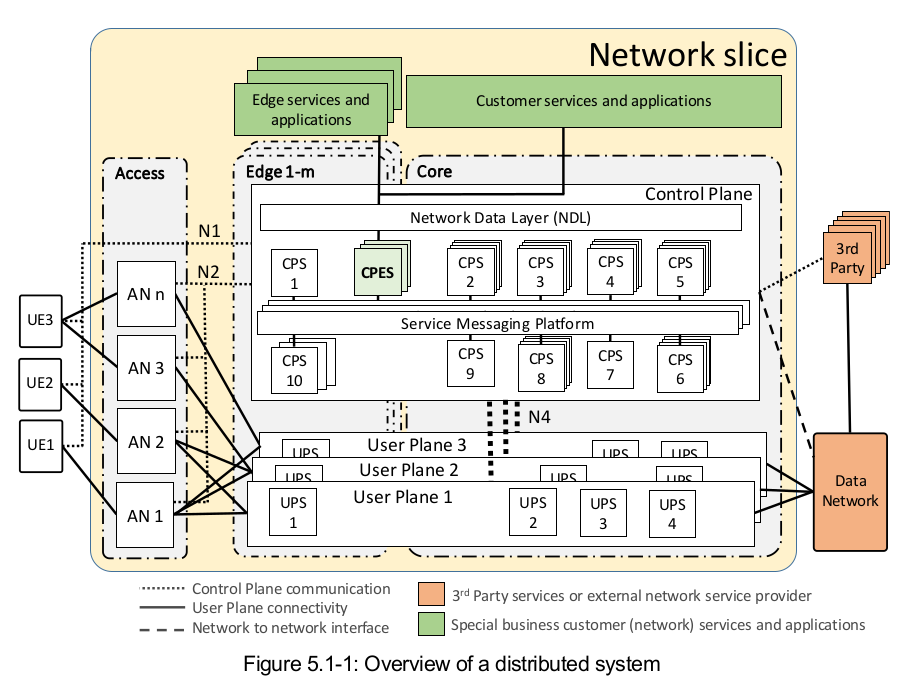
\includegraphics[width=0.9\textwidth]{images/distributed-sba}
\end{frame}

\begin{frame}
  \frametitle{Roaming with slice spaning accross domains}
  \center
  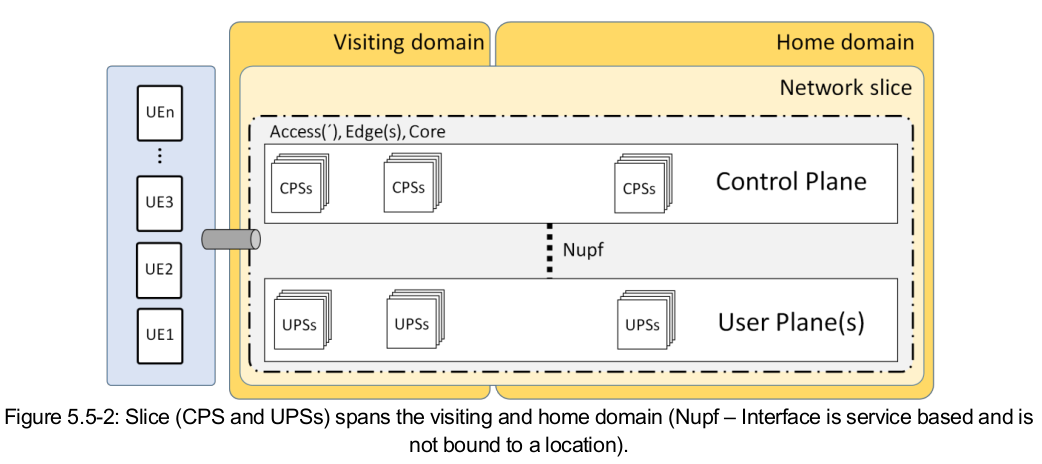
\includegraphics[width=0.9\textwidth]{images/sba-roaming}
\end{frame}



\begin{frame}
  \frametitle{SBA platform}
  \begin{itemize}
    \item push common patterns from service layer to platform layer (service registration/discovery, external service exposure)
    \item {separate Dev/Ops; foster multi-vendor developments}
  \end{itemize}
  \center
  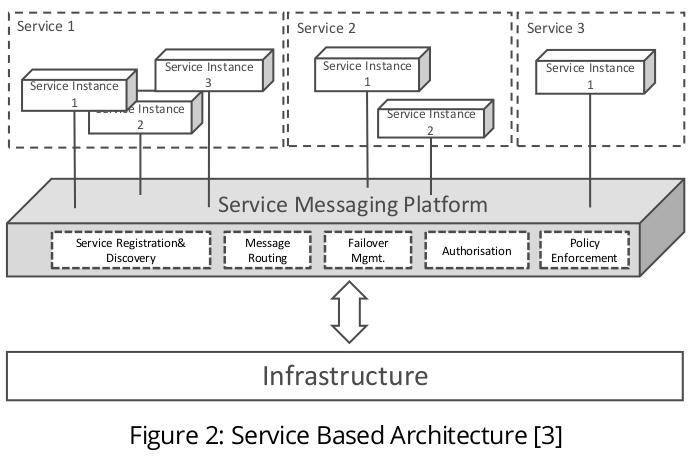
\includegraphics[width=0.9\textwidth]{images/cn-sba}
\end{frame}

\begin{frame}
  \frametitle{Centralized Bus implementation}
  \center
  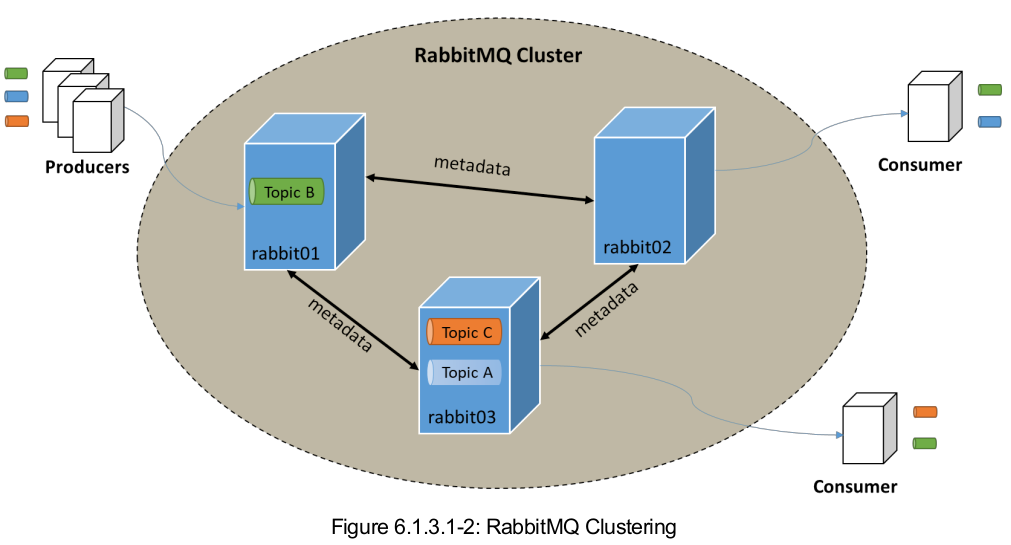
\includegraphics[width=0.9\textwidth]{images/rabitmq}
\end{frame}

\begin{frame}
  \frametitle{Distributed message routing architechture (SCP)}
  It seems it is similar to sidecar service mesh architechture (istio + envoy)
  \center
  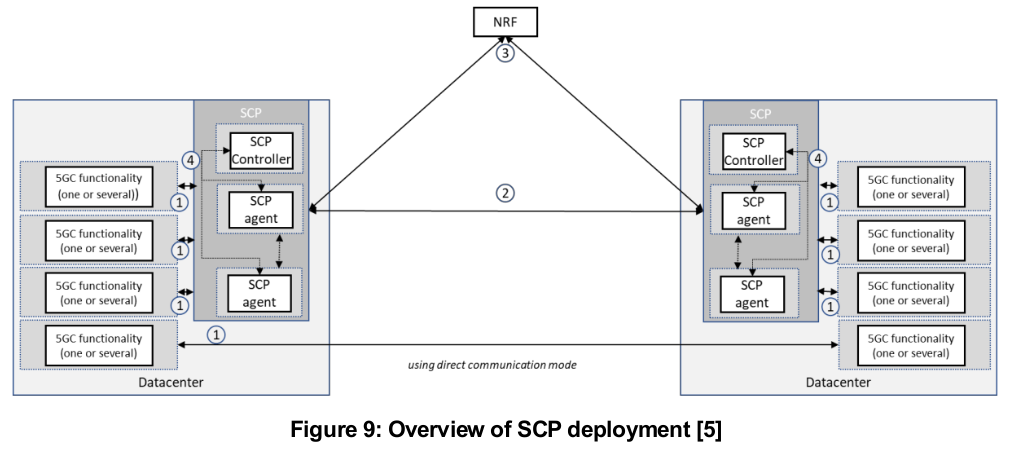
\includegraphics[width=0.9\textwidth]{images/scp-deploy}
\end{frame}

\begin{frame}
  \frametitle{FUDGE-5G}
  \begin{center}
  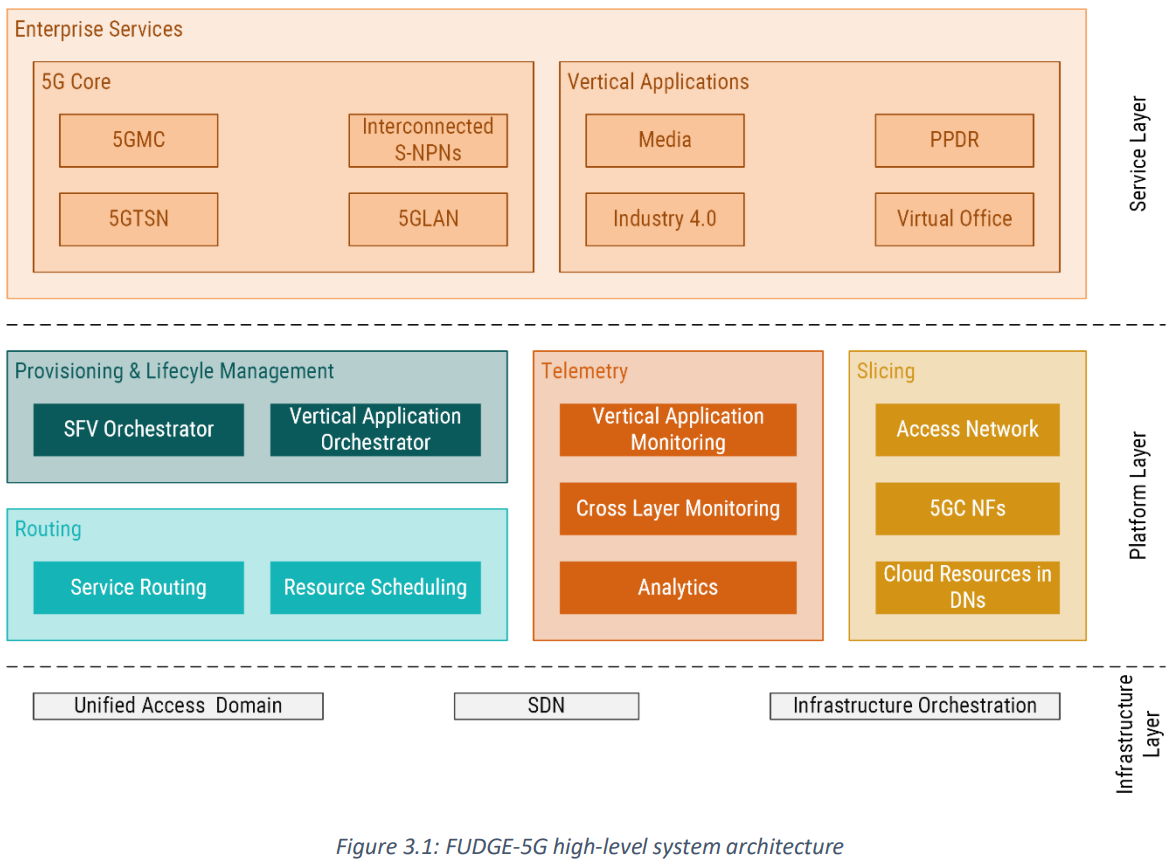
\includegraphics[width=0.8\textwidth]{images/fudge-5g}
  \end{center}
  \small Unified Service-based Architecture placing service
registration, routing, orchestration and resource control at the
platform level with 5GC and vertical applications as 5G
services on top of platform
\end{frame}

\begin{frame}
  \center
  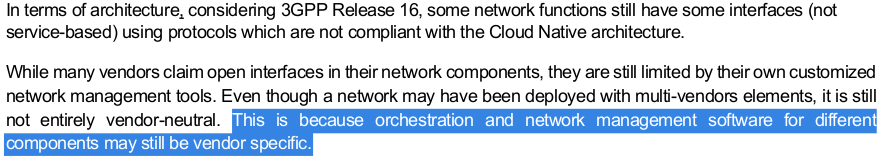
\includegraphics[width=\textwidth]{images/cn-challenges}
\end{frame}

\begin{frame}
  \frametitle{Hybrid cloud deployment}
  \center
  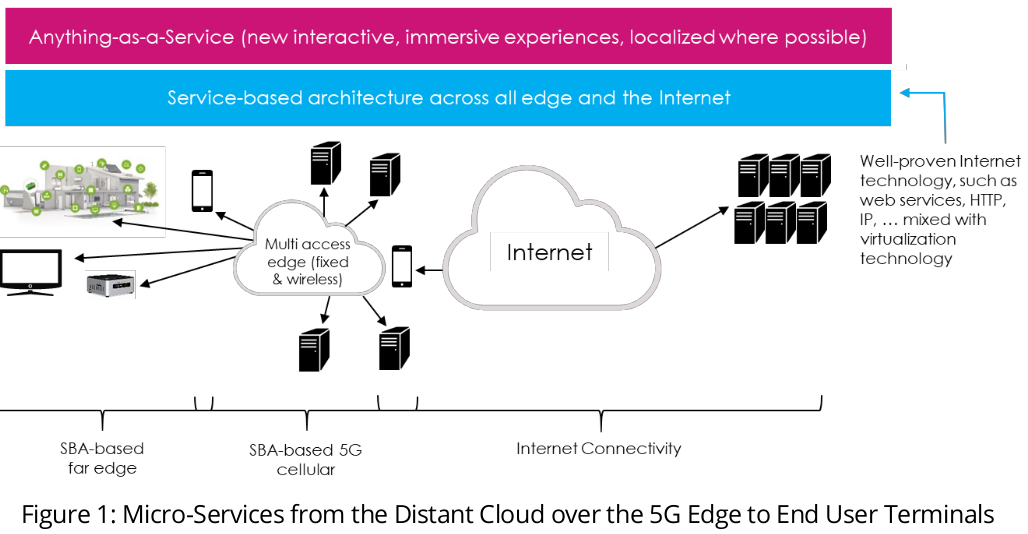
\includegraphics[width=\textwidth]{images/sbi-hybridcloud}
\end{frame}

\begin{frame}
  \frametitle{Name-based routing SCP}
  \center
  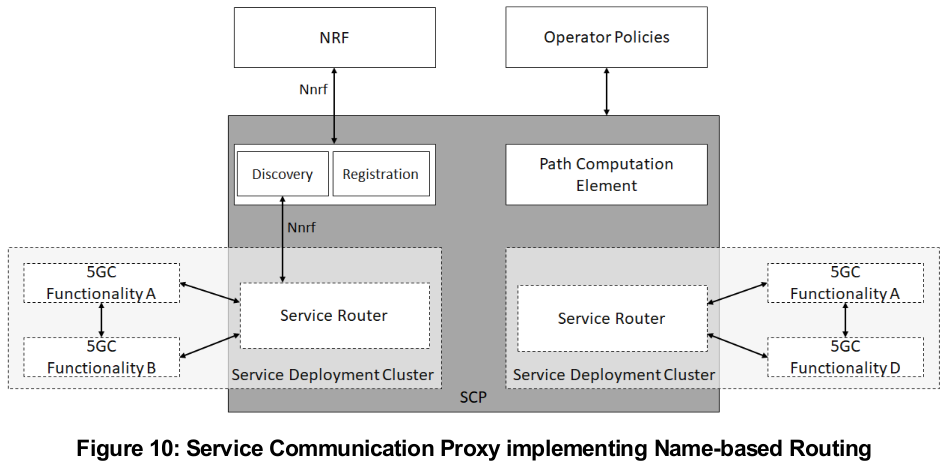
\includegraphics[width=0.9\textwidth]{images/scp-nbr-deploy}
\end{frame}
\begin{frame}
  \frametitle{Name-based routing architechture (SDN-based ICN flavor)}
  \center
  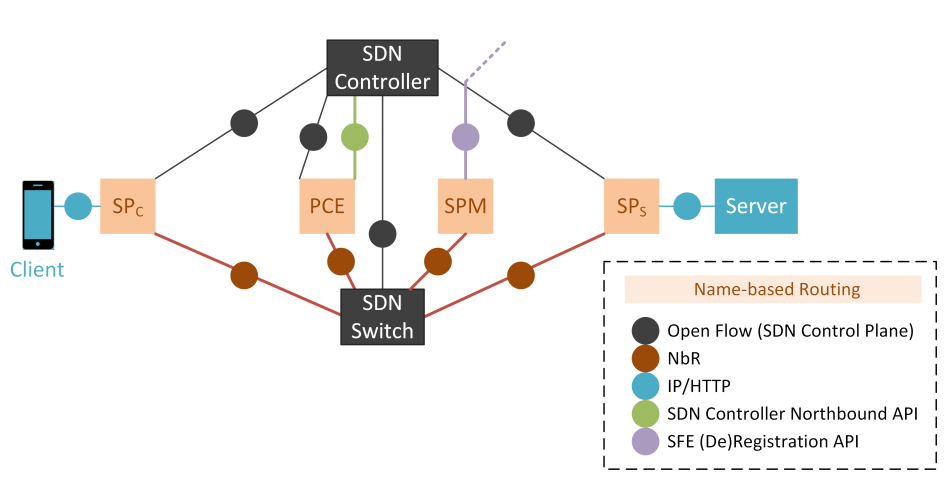
\includegraphics[width=0.9\textwidth]{images/nbr}
\end{frame}



\begin{frame}
  \frametitle{}
  \center
  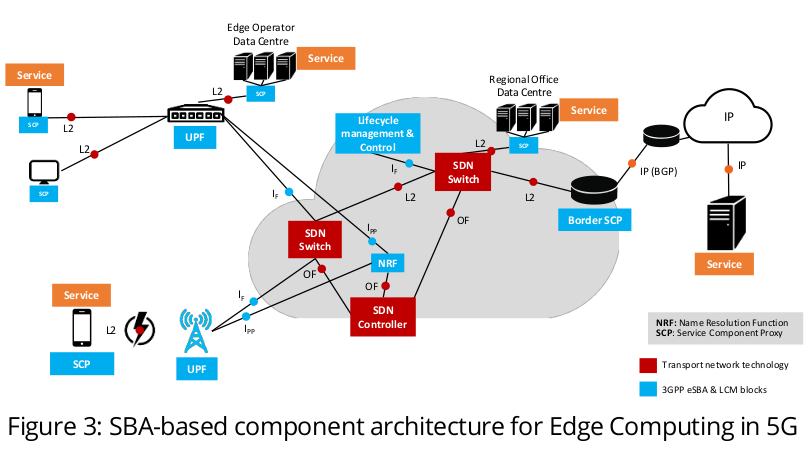
\includegraphics[width=0.9\textwidth]{images/fudge-esba}
\end{frame}
\begin{frame}
  \frametitle{Interconnected NPN use case}
  \center
    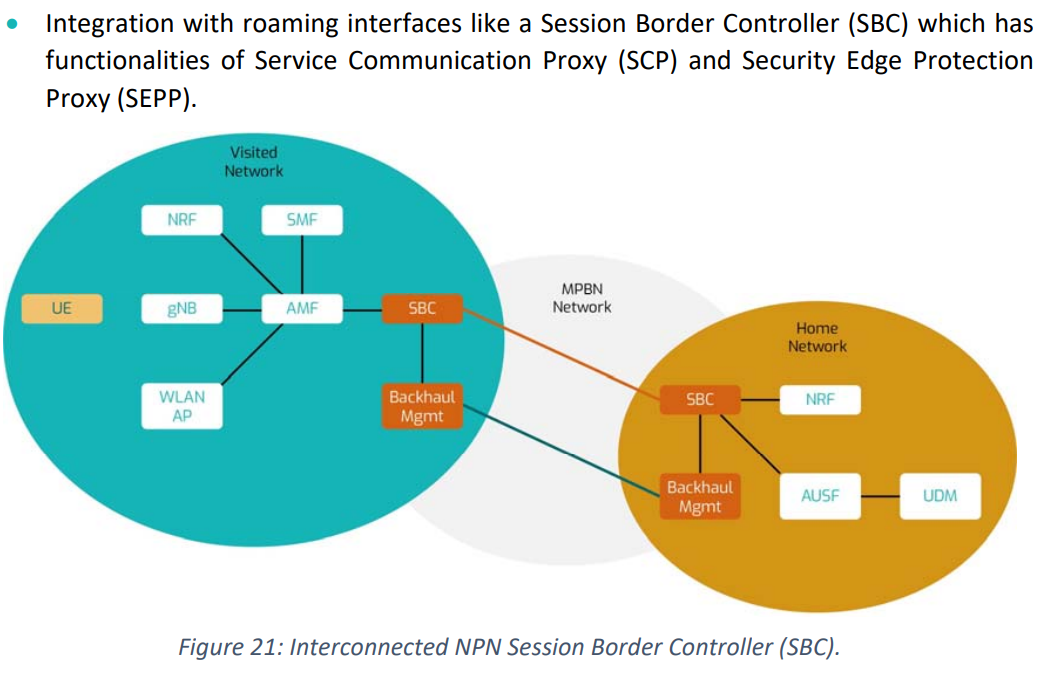
\includegraphics[width=\textwidth]{images/scp-roaming}
\end{frame}

\begin{frame}
  \frametitle{Realizing the unified SBA platform}
  \begin{itemize}
    \item {Kubernetes + Istio + Evoy can build a domain SBA plaform. To build a unified SAB accross different domains, we may need to do more research}
    \item {FUDGE-5G proposed Name-Based routing SCP}
    \item {NDN flavor based SCP?}    
  \end{itemize}
\end{frame}

\begin{comment}
\begin{frame}
  \frametitle{Cloud-native definition}
  Cloud native technologies empower organizations to build and run scalable applications in modern, dynamic environments such as public, private, and hybrid clouds. Containers, service meshes, microservices, immutable infrastructure, and declarative APIs exemplify this approach. (CNCF)
\end{frame}
\end{comment}

\begin{frame}
  \Large{2022/06/23 $\rightarrow$}
\end{frame}



\begin{frame}
  \frametitle{Separate business logic and operation}
\end{frame}

\begin{frame}
  \frametitle{Network Slice as a Service}
  \center
  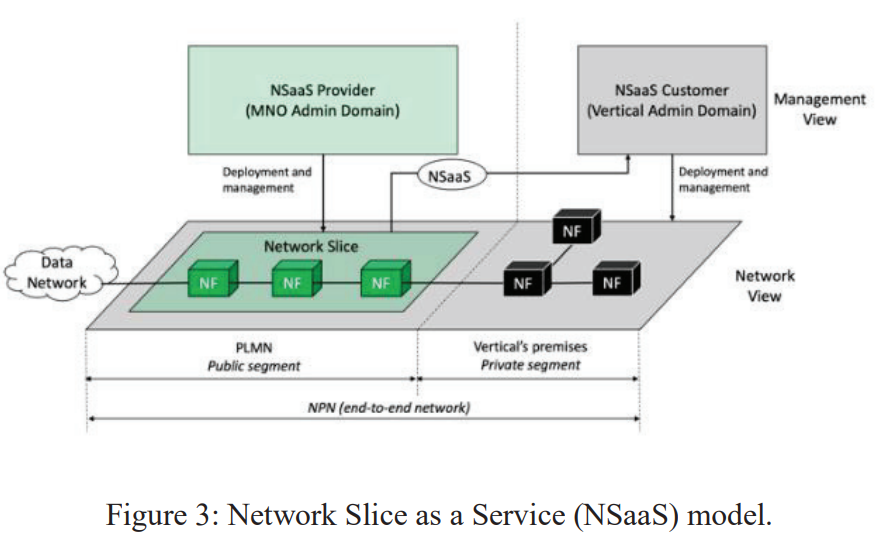
\includegraphics[width=0.9\textwidth]{images/ns-as-a-service}
  \tiny Wint Yi Poe et.al. "Provisioning Private 5G networks by means of
Network Slicing: Architectures and Challenges"
\end{frame}
 

\begin{frame}
  \frametitle{Slice compose}
  \center
  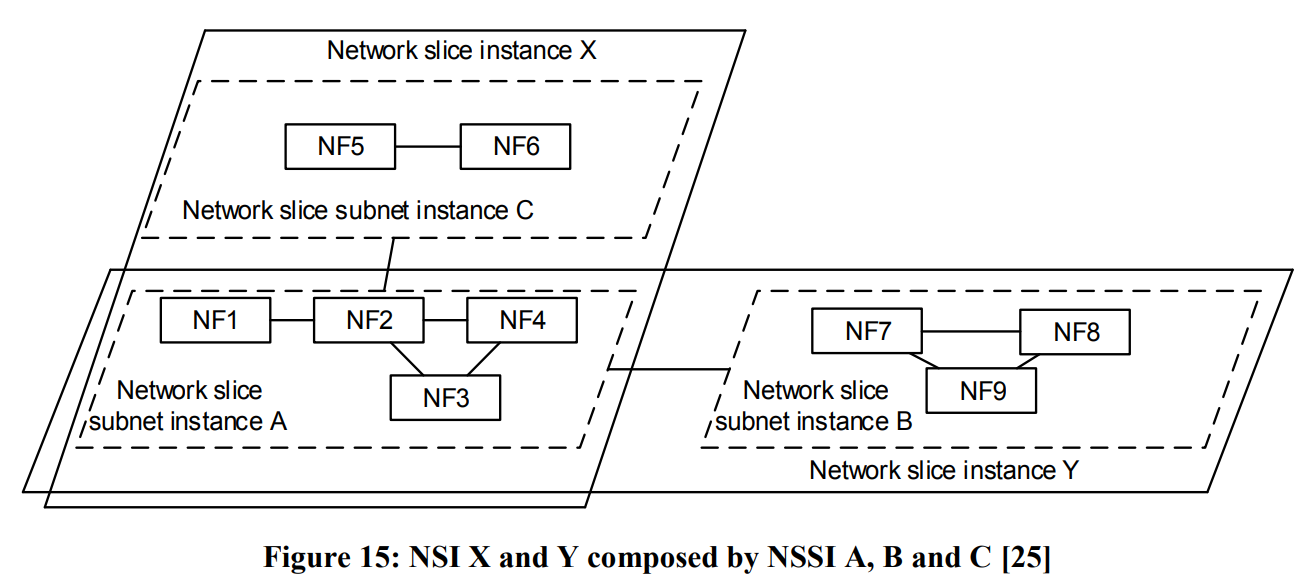
\includegraphics[width=0.9\textwidth]{images/ns-compose}
  
  \href{https://zenodo.org/record/3628333\#.YrLzD3XP2EJ}{\tiny{5G EVE end to end facility reference architecture for vertical industries and core applications}}
\end{frame}

\begin{frame}
  \frametitle{Slice compose}
  \center
  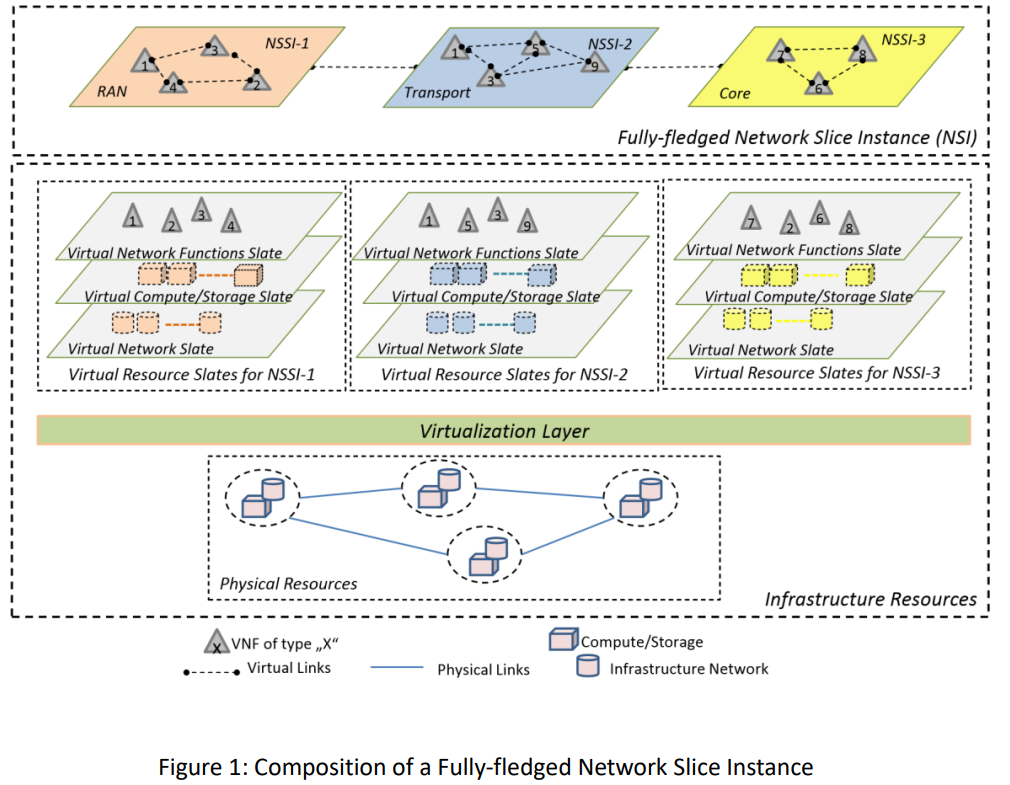
\includegraphics[width=0.9\textwidth]{images/ns-compose1}
  
  \tiny {Tarik Taleb et.al. "On Multi-domain Network Slicing Orchestration
Architecture \& Federated Resource Control"}

\end{frame}


\begin{frame}
  \frametitle{multi-domain network slicing architechture}
  \center
  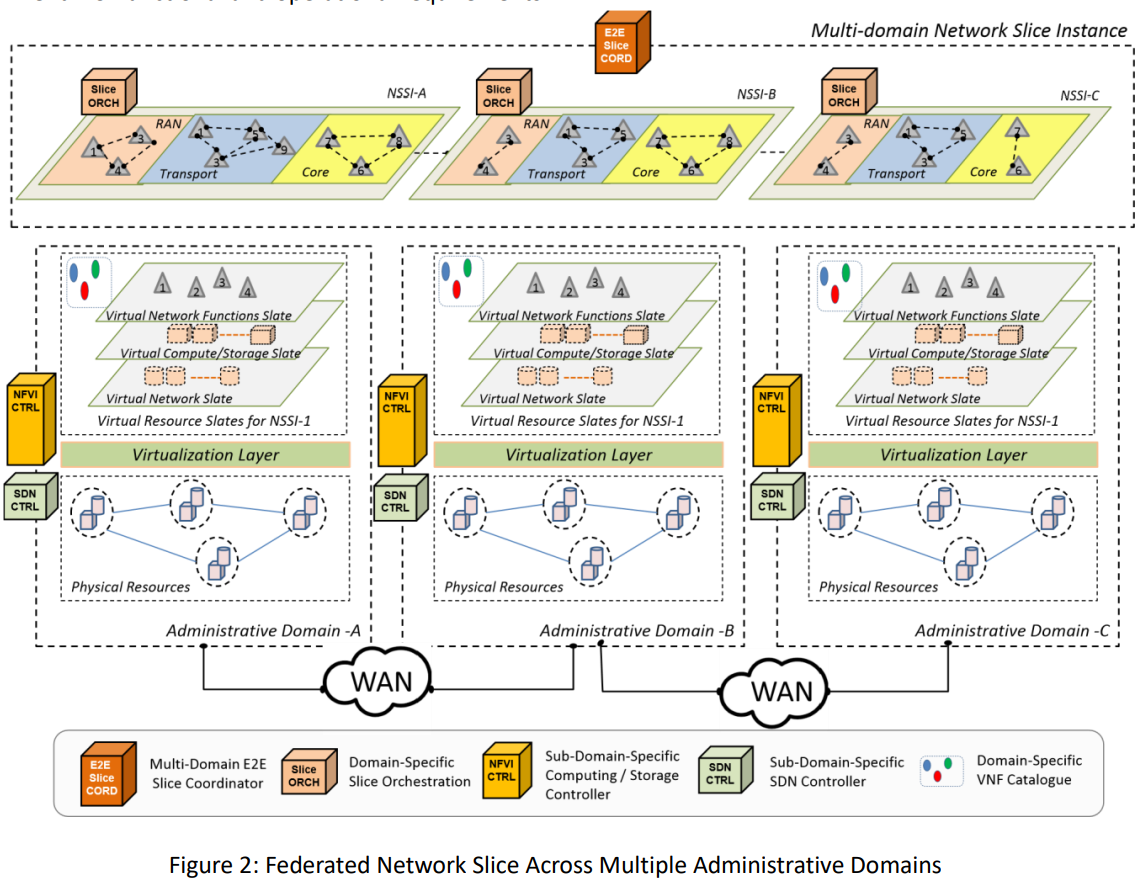
\includegraphics[width=0.9\textwidth]{images/ns-compose-arch}
  
  \tiny {Tarik Taleb et.al. "On Multi-domain Network Slicing Orchestration
Architecture \& Federated Resource Control"}

\end{frame}

\begin{frame}
  \frametitle{Network function selection issues}
  \begin{center}
    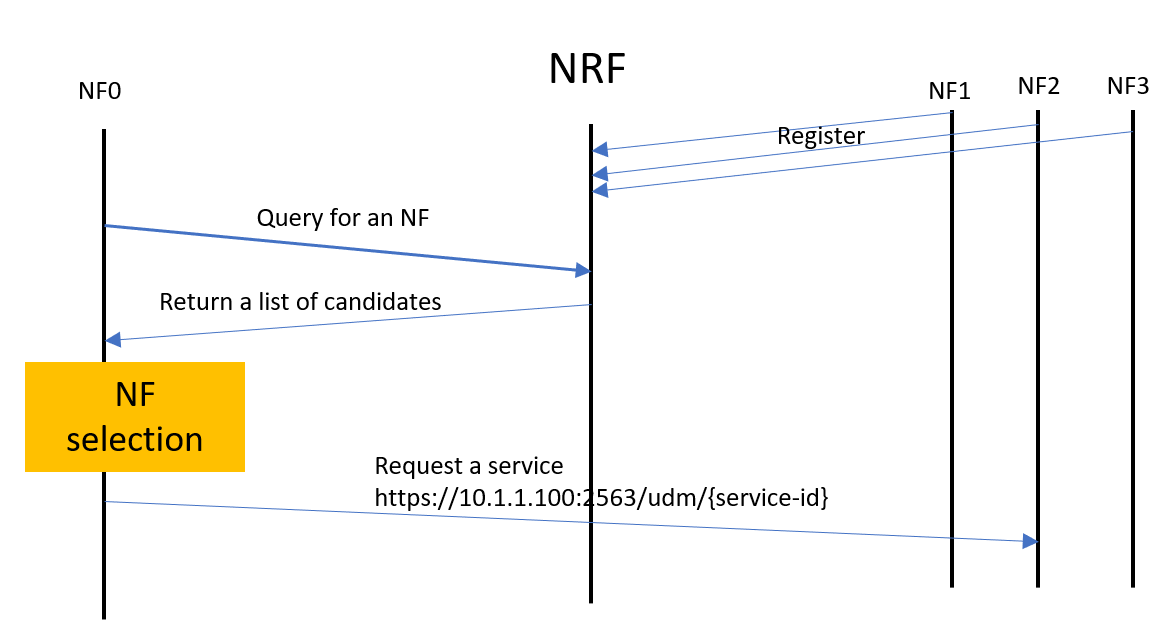
\includegraphics[width=0.8\textwidth]{images/nf-selection}  
  \end{center}    
  \begin{itemize}
    \item {NF selection is hardwired to bussiness logic implementation $\rightarrow$ vendor specific}
    \item {NF selection encloses load balancing, fault tolerence, resiliency etc. $\rightarrow$ bussiness logic is intefered with operations}
    \item {SCP is still defined as an optinal network function. Its implementation is still vendor specific}
  \end{itemize}
\end{frame}
\begin{frame}
  \frametitle{Cross-domain service requesting}
  How to look for an SMF?
  \begin{itemize}
    \item Which domain to look for?
    \item Needs a right to query that NRF
    \item Ask the NRF of that domain for a list of SMF candidates
    \item Select an SMF which I have a right to request
  \end{itemize}
  The logic is complex
\end{frame}

\begin{frame}
  \frametitle{Let the service messaging platform handle NF selection}
  \begin{center}
    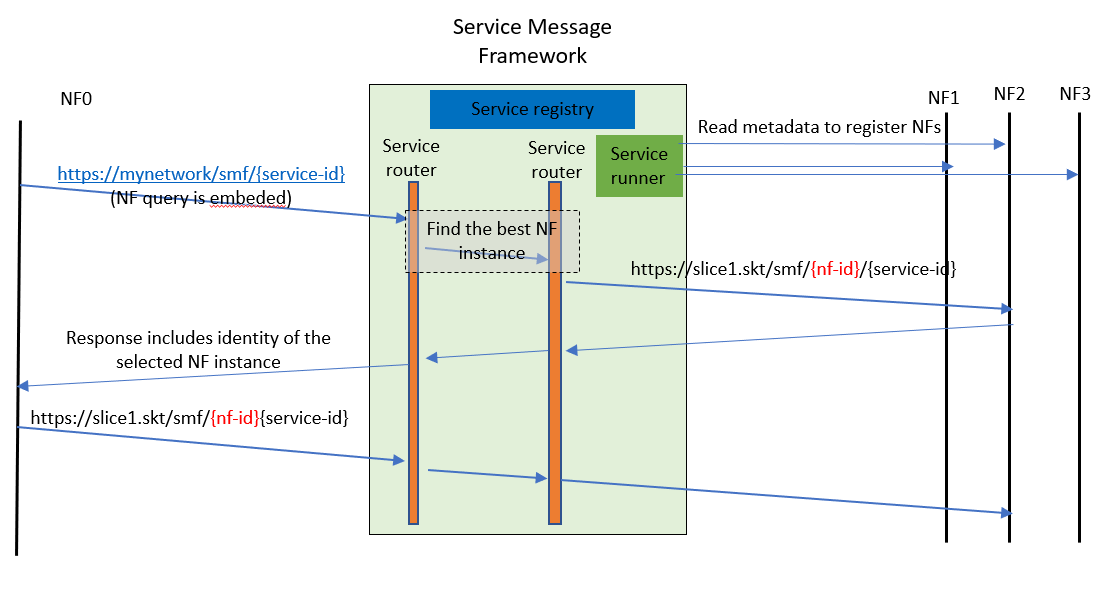
\includegraphics[width=0.8\textwidth]{images/smp}
  \end{center}
  \begin{itemize}
    \item seperate bussiness logic from deployment/operation; bussiness logic is much more simple
    \item the platform should do NF selection better becuase it has a global view of the system
    \item a service has a unique name. There can be multiple instances (with different identity) for a same service.
  \end{itemize}
\end{frame}

\begin{frame}
  \frametitle{A service messaging platform for multi-domain slicing network}
  \begin{center}
    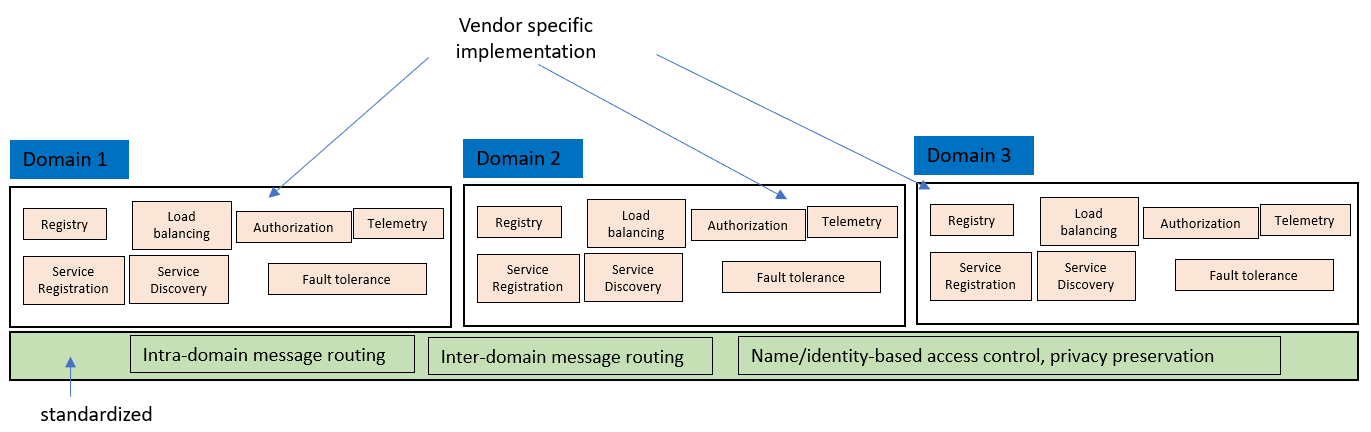
\includegraphics[width=\textwidth]{images/multi-domain-smp}
  \end{center}
\end{frame}

\begin{frame}
  \frametitle{Naming scheme}
  \begin{center}
    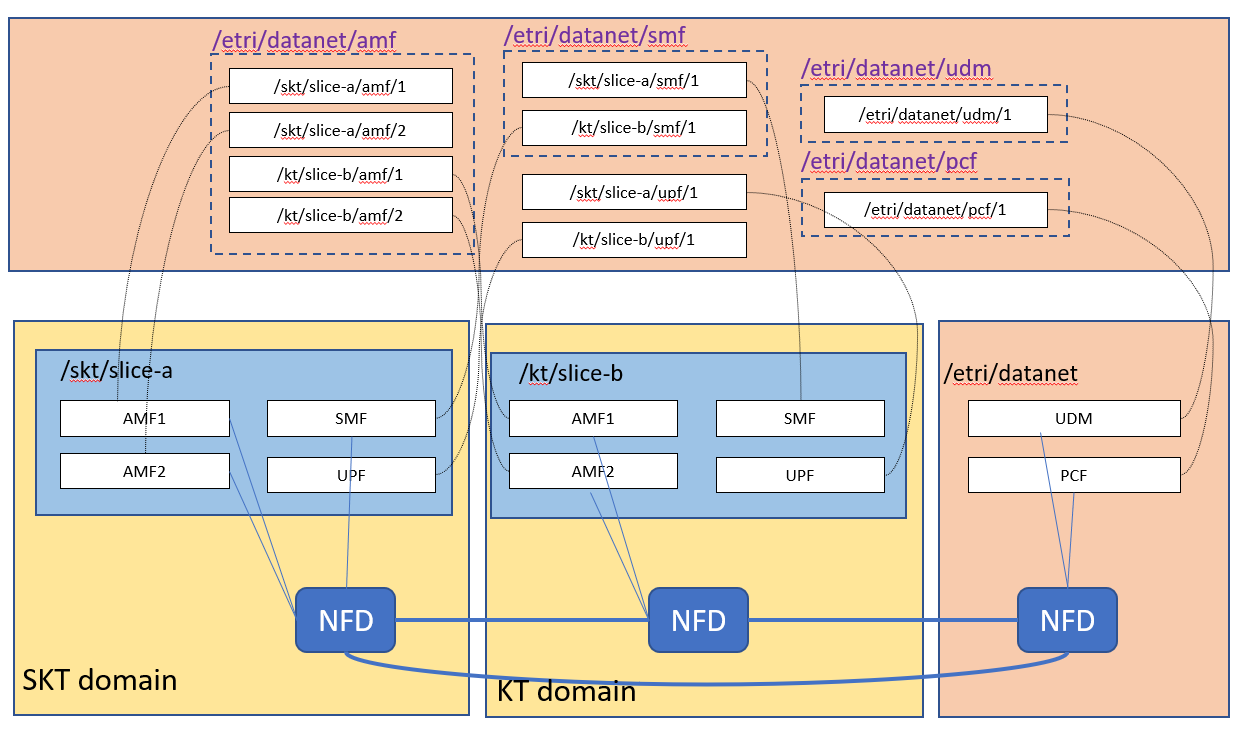
\includegraphics[width=0.9\textwidth]{images/slice-naming}
  \end{center}
\end{frame}

\begin{frame}
  \frametitle{Envoy architechture}
  Envoy is an L7 proxy and communication bus designed for large modern service oriented architectures. The project was born out of the belief that:

  \begin{quote}\small The network should be transparent to applications. When network and application problems do occur it should be easy to determine the source of the problem.
  \end{quote}
  \center
  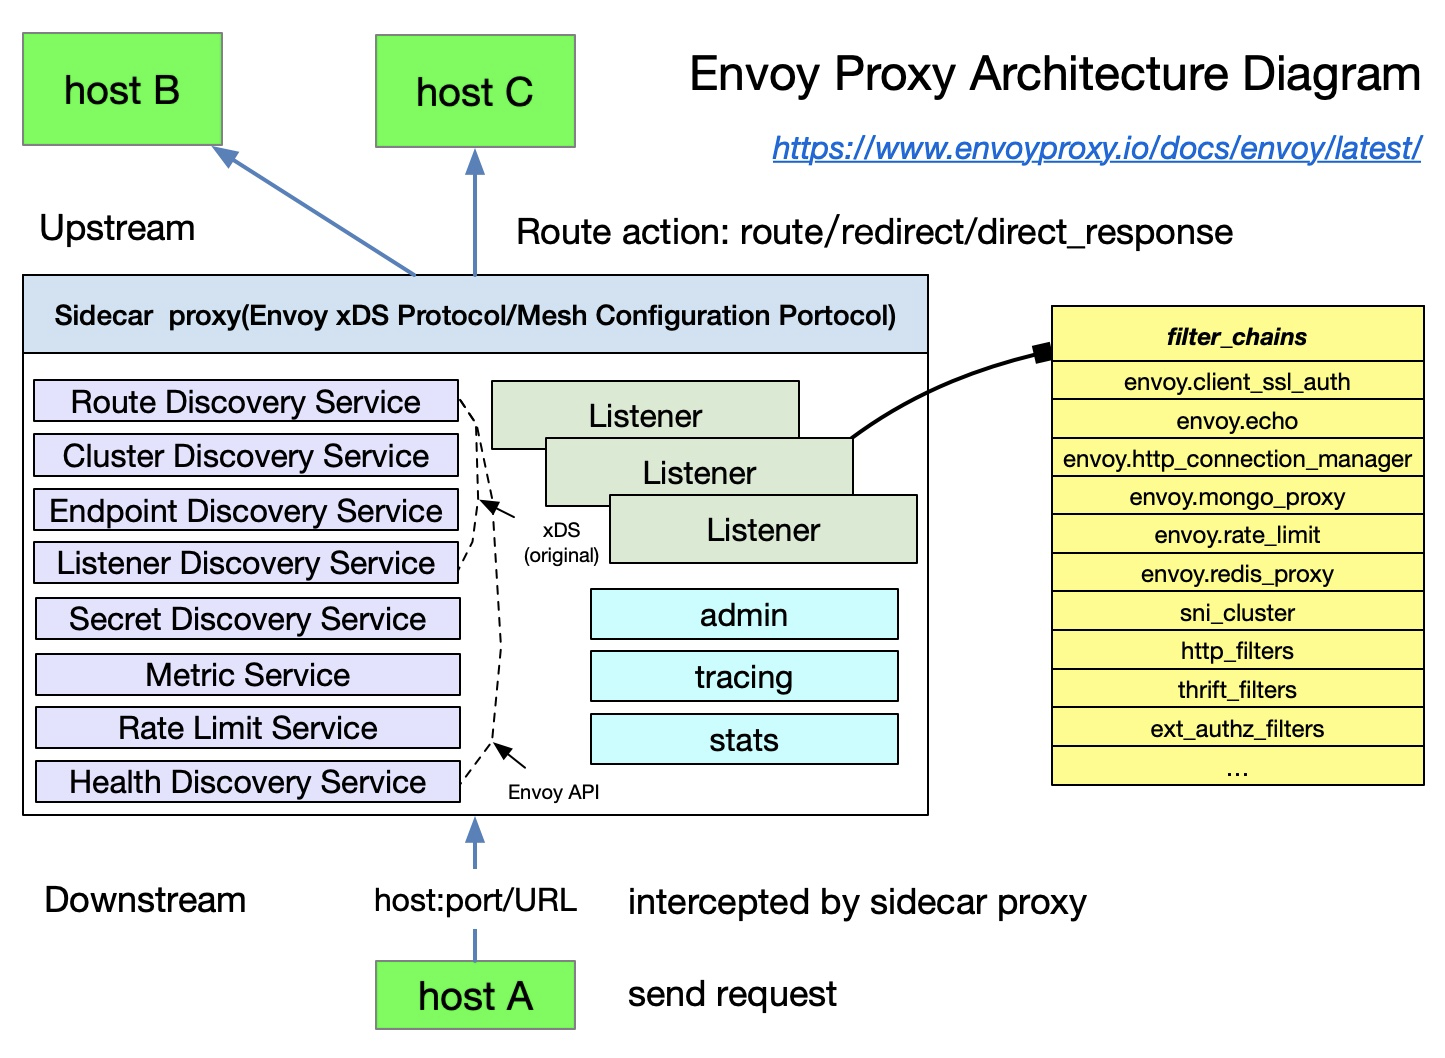
\includegraphics[width=0.7\textwidth]{images/envoy-arch}
\end{frame}

\begin{frame}
  \frametitle{Envoy (sidecar) limitation}
  \begin{itemize}
    \item {Complexity}
    \item {Latency (can be a big problem for 5G/6G signaling)}
  \end{itemize}
  \begin{center}
    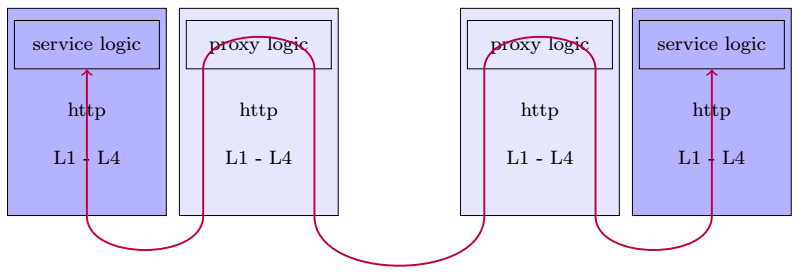
\includegraphics[width=0.7\textwidth]{images/envoy-latency}
  \end{center}
  
\end{frame}

\begin{frame}
  \frametitle{Native envoy for 5g core network function}
  envoy as a library instead of a sidecar application (envoylite)
  \begin{itemize}
    \item {Service registration/discovery, security, NF selection, and telemetry is moved to envoylite. Isolate them from the NF's business logic}
    \item {Talk to a service mesh (istio/linkerd etc)}
    \item {Have a common gateway connecting  service meshes (service mesh agnotic); name-based routing}
  \end{itemize}
  \center
  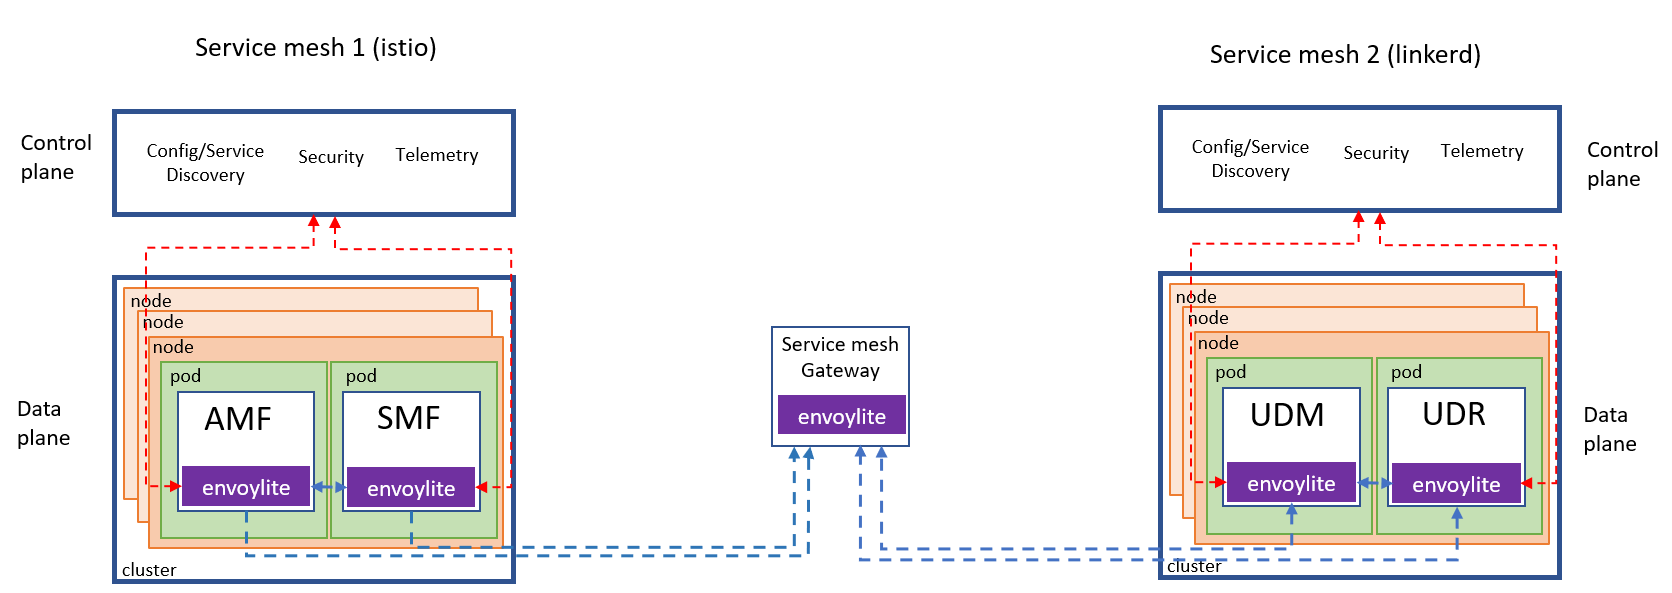
\includegraphics[width=\textwidth]{images/envoylite}
\end{frame}

\begin{frame}
  \frametitle{envoylite over ???}
  \center
  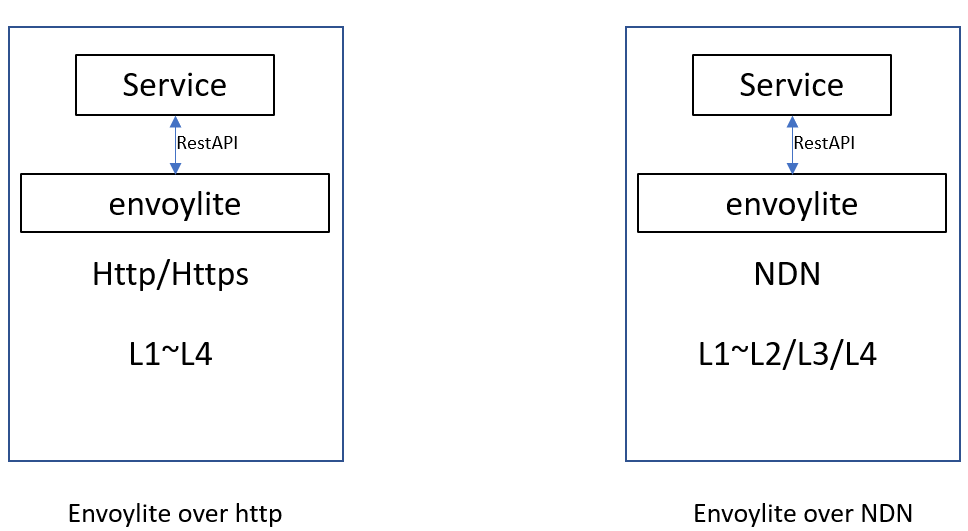
\includegraphics[width=\textwidth]{images/envoylite-stack}
\end{frame}
\end{document}
